\documentclass[11pt,a4paper]{article}
\usepackage[margin=1in]{geometry}
\usepackage{amsmath,amssymb,amsthm,mathtools,bm}
\usepackage{enumitem}
\usepackage{booktabs}
\usepackage{array}
\usepackage{xcolor}
\usepackage{hyperref}
\usepackage{tikz}
\usetikzlibrary{arrows.meta,positioning,calc,decorations.pathreplacing,shapes.geometric}
\hypersetup{colorlinks=true,linkcolor=blue,urlcolor=blue,citecolor=blue}
\setlist[itemize]{leftmargin=2em,itemsep=0.3em,topsep=0.35em}
\setlist[enumerate]{leftmargin=2.2em,itemsep=0.3em,topsep=0.35em}

\newcommand{\R}{\mathbb{R}}
\newcommand{\N}{\mathbb{N}}
\newcommand{\ReLU}{\operatorname{ReLU}}
\newcommand{\Conv}{\operatorname{Conv}}
\newcommand{\Span}{\operatorname{span}}
\newcommand{\dd}{\,\mathrm{d}}
\newcommand{\Th}{\mathcal{T}_h}
\newcommand{\Vh}{V_h}
\newcommand{\Ah}{A_{\mathrm{Hat}}}
\newcommand{\Ar}{A_{\mathrm{ReLU}}}
\newcommand{\argmin}{\operatorname*{arg\,min}}

\definecolor{titleblue}{RGB}{22,74,135}
\definecolor{softblue}{RGB}{235,244,255}
\definecolor{softgray}{RGB}{245,245,245}
\definecolor{softgreen}{RGB}{236,249,239}

\theoremstyle{definition}
\newtheorem{definition}{Definition}[section]
\newtheorem{example}{Example}[section]
\theoremstyle{plain}
\newtheorem{theorem}{Theorem}[section]
\newtheorem{proposition}{Proposition}[section]
\newtheorem{lemma}{Lemma}[section]
\theoremstyle{remark}
\newtheorem{remark}{Remark}[section]

\newcommand{\boxnote}[1]{%
  \vspace{0.5em}
  \noindent\colorbox{softblue}{\parbox{0.965\linewidth}{#1}}
  \vspace{0.5em}
}
\newcommand{\supplement}[1]{%
  \vspace{0.5em}
  \noindent\colorbox{softgreen}{\parbox{0.965\linewidth}{\textbf{Supplement from the complete slides.} #1}}
  \vspace{0.5em}
}

\title{\textbf{Revised and Expanded Lecture Notes\\Deep Neural Networks and Finite Element Methods}}
\author{Prepared from the classroom notes and the complete course slides}
\date{July 6--7, 2026}

\begin{document}
\maketitle
\tableofcontents
\newpage

\section*{Revision Note}
\addcontentsline{toc}{section}{Revision Note}
The earlier version of these notes was reconstructed from classroom photographs. The present version compares that draft with the complete slide decks \emph{Topic 0: Introduction} and \emph{Topic 1: Finite Element and Neural Networks}. Material already contained in the earlier notes has been checked and expanded in place. Topics that were absent from the photographs are collected in later sections, especially the scientific context of deep learning, the complete finite element derivation, convergence estimates, gradient descent, and the universal approximation theorem.

\subsection*{Comparison with the earlier draft}
\begin{center}
\renewcommand{\arraystretch}{1.25}
\begin{tabular}{p{0.29\linewidth}p{0.60\linewidth}}
\toprule
\textbf{Already present} & \textbf{Added or corrected from the complete slides}\\
\midrule
Course policies and objectives & Schedule, staff, prerequisites, course materials, tests, grading, and prizes.\\
Hiring example and ReLU salary model & One-factor threshold model, numerical candidate tables, and the motivation for learning parameters from data.\\
DNN composition and supervised learning & Artificial-neuron notation, common activations, one-hot classification, population versus empirical risk, and gradient descent.\\
Finite element algebraic system & Model PDE, weak formulation, energy minimization, Galerkin method, C\'ea's lemma, and the $H^1$ error estimate.\\
Hat/ReLU correspondence & Exact one-dimensional stiffness matrices and a complete matrix proof of $\Ar=\Ah^{-1}$.\\
Meshes, barycentric coordinates, nodal bases & Higher-dimensional shallow networks, $\ReLU^k$ networks, and universal approximation.\\
\bottomrule
\end{tabular}
\end{center}

\section{Course Information, Policies, and Objectives}

\subsection{Basic information}
The course is \emph{Mathematical Theory for Deep Neural Networks}, taught at Peking University from July 6 to July 17, 2026, Monday through Friday, 09:00--11:00. The instructor is Professor Jinchao Xu. The class email is \texttt{ai@multigrid.org}.

The lectures combine two components:
\begin{itemize}
  \item mathematical motivation, description, and analysis of deep learning algorithms;
  \item hands-on programming exercises for representative models.
\end{itemize}
The course materials consist of slides, related research papers, and programming subroutines. The listed prerequisites are multivariable calculus, linear algebra, basic numerical analysis, and some Python experience.

\subsection{Policies}
\begin{itemize}
  \item Bring the name card to every class.
  \item Homework is assigned after each class and is due before the next class. A PDF is submitted to \texttt{ai@multigrid.org}.
  \item Two tests are held at the end of each week.
  \item The final grade depends on both homework and test scores.
\end{itemize}
The slides also list certificates and prizes for the best students.

\subsection{Objectives}
The two main objectives are:
\begin{enumerate}
  \item to provide a mathematical understanding of how and why deep learning works;
  \item to provide programming experience with deep neural networks, convolutional neural networks, Transformers, and related models.
\end{enumerate}

\section{From Intelligence and Decision Rules to Neural Networks}

\subsection{Natural and artificial intelligence}
The introduction distinguishes the following ideas:
\begin{itemize}
  \item intelligence is the ability to learn, understand, and judge;
  \item natural intelligence exists in nature;
  \item artificial intelligence is intelligence expressed by machines and computer programs designed by humans.
\end{itemize}
The purpose of the course is not only to use artificial intelligence, but also to identify the mathematical structures behind it.

\subsection{A one-factor decision rule}
Let $x$ be years of experience. A simple hiring rule is
\[
  x>3 \Longrightarrow \text{Yes},
  \qquad
  x\le 3 \Longrightarrow \text{No}.
\]
With the Heaviside function
\[
  H(s)=
  \begin{cases}
    1,&s>0,\\
    0,&s\le 0,
  \end{cases}
\]
this rule can be written as
\[
  y=H(Wx+b),\qquad W=1,\quad b=-3.
\]
Thus even a very simple decision rule already has the form ``affine map followed by a nonlinear activation.''

\subsection{A linear score based on two factors}
Suppose a candidate is described by
\[
  x_1=\text{experience (years)},\qquad x_2=\text{education (degree)}.
\]
Let
\[
  x=\begin{pmatrix}x_1\\x_2\end{pmatrix},
  \qquad
  W=\begin{pmatrix}w_1&w_2\end{pmatrix}.
\]
The score is
\[
  s(x)=w_1x_1+w_2x_2+b=Wx+b,
\]
and the binary decision is $y=H(s(x))$.

For the concrete choice
\[
  w_1=1,\qquad w_2=2,\qquad b=-5,
\]
the score is $x_1+2x_2-5$. The example in the slides gives:
\begin{center}
\begin{tabular}{ccccc}
\toprule
Candidate & Years & Degree value & Score & Decision\\
\midrule
1 & 3 & 4 & 6 & Yes\\
2 & 6 & 2 & 5 & Yes\\
3 & 4 & 1 & 1 & Yes\\
4 & 1 & 2 & 0 & No\\
\bottomrule
\end{tabular}
\end{center}
The limitation is that $H$ only produces the two values $0$ and $1$.

\subsection{Using ReLU for a continuous output}
The ReLU activation is
\[
  \ReLU(s)=\max\{0,s\}=
  \begin{cases}
    s,&s>0,\\
    0,&s\le 0.
  \end{cases}
\]
A salary model may be written as
\[
  y=W^1\ReLU(W^0x+b^0).
\]
For $W^1=2000$ and the same score $x_1+2x_2-5$,
\[
  y=2000\ReLU(x_1+2x_2-5).
\]
The four candidates above receive the values $12000$, $10000$, $2000$, and $0$, respectively.

\begin{center}
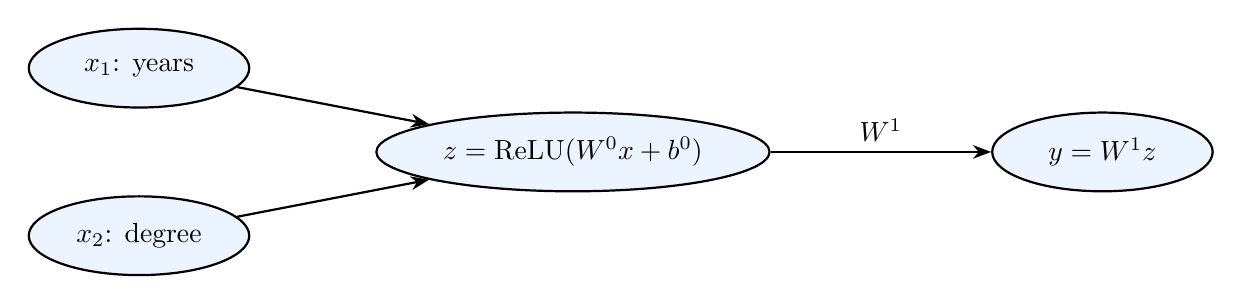
\begin{tikzpicture}[>=Stealth,node distance=2.0cm]
  \tikzstyle{oval}=[ellipse,draw,thick,minimum width=2.8cm,minimum height=1.0cm,fill=softblue]
  \node[oval] (x1) {$x_1$: years};
  \node[oval,below=1.1cm of x1] (x2) {$x_2$: degree};
  \node[oval,right=3.0cm of $(x1)!0.5!(x2)$] (h) {$z=\ReLU(W^0x+b^0)$};
  \node[oval,right=2.8cm of h] (y) {$y=W^1z$};
  \draw[->,thick] (x1) -- (h);
  \draw[->,thick] (x2) -- (h);
  \draw[->,thick] (h) -- node[above] {$W^1$} (y);
\end{tikzpicture}
\end{center}

\subsection{A more refined model}
With five raw features,
\[
  x^0=x=(x_1,\ldots,x_5)^T,
\]
where the entries denote years, management experience, degree, university rank, and GPA, the first hidden layer can form two intermediate features:
\[
  x^1=\ReLU(W^0x+b^0),
\]
with
\[
  W^0=
  \begin{pmatrix}
    w_{11}^0&w_{12}^0&0&0&0\\
    0&0&w_{23}^0&w_{24}^0&w_{25}^0
  \end{pmatrix}.
\]
The first row represents an experience feature and the second row an education feature. Further composition gives
\[
  x^2=\ReLU(W^1x^1+b^1),\qquad y=W^2x^2.
\]
This is already a deep neural network.

\section{Artificial Neurons and Deep Neural Networks}

\subsection{Linear maps and activation functions}
For $x\in\R^m$, a vector-valued affine map has the form
\[
  Wx+b=
  \begin{pmatrix}
    W_1x+b_1\\
    \vdots\\
    W_nx+b_n
  \end{pmatrix},
  \qquad
  W_kx+b_k=\sum_{i=1}^m w_{k,i}x_i+b_k.
\]
Common activation functions in the slides are
\[
  H(x),\qquad \frac{1}{1+e^{-x}},\qquad \ReLU(x)=\max(0,x).
\]
An artificial neuron consists of an affine transformation $\theta(x)=Wx+b$ and a nonlinear activation $\sigma$; its output is
\[
  y=\sigma(\theta(x)).
\]

\subsection{Composition and network depth}
Let $n_0=d$ be the input dimension and let $n_1,\ldots,n_L$ be hidden-layer widths. Set
\[
  x^{(0)}=x,
  \qquad
  x^{(\ell+1)}=\sigma\bigl(W^\ell x^{(\ell)}+b^\ell\bigr),
  \quad \ell=0,\ldots,L-1.
\]
The final output layer is
\[
  f(x;\Theta)=W^Lx^{(L)}+b^L.
\]
Here
\[
  W^\ell\in\R^{n_{\ell+1}\times n_\ell},
  \qquad b^\ell\in\R^{n_{\ell+1}},
\]
and $\Theta$ denotes all weights and biases. A DNN is an artificial neural network with multiple layers.

\boxnote{The mathematical structure of a DNN is repeated composition: affine map, nonlinear activation, affine map, nonlinear activation, and so on. Depth records the number of such stages, while width records the number of neurons in each stage.}

\section{Learning from Data}

\subsection{Regression-style formulation}
Suppose the training data are
\[
  \{(x^i,y^i)\}_{i=1}^N.
\]
In the employee example, $x^i$ contains experience and education, and
\[
  y^i\in\{0,1,2,3,4\}
\]
represents the levels bad, fair, good, very good, and excellent. Learning means choosing parameters so that
\[
  f(x^i;\Theta)\approx y^i.
\]
For the squared loss,
\[
  L_N(\Theta)=\frac1N\sum_{i=1}^N\left|f(x^i;\Theta)-y^i\right|^2,
  \qquad
  \Theta^*=\argmin_\Theta L_N(\Theta).
\]
A new sample is then evaluated by $f(x^{\mathrm{new}};\Theta^*)$.

\subsection{Classification and one-hot labels}
For three classes such as cat, dog, and rabbit, the targets may be written as
\[
  e_1=\begin{pmatrix}1\\0\\0\end{pmatrix},\qquad
  e_2=\begin{pmatrix}0\\1\\0\end{pmatrix},\qquad
  e_3=\begin{pmatrix}0\\0\\1\end{pmatrix}.
\]
A network output such as
\[
  f(x;\Theta)=\begin{pmatrix}0.7\\0.2\\0.1\end{pmatrix}
\]
is interpreted as class $1$ because its first component is largest.

An image is represented numerically as a large array of pixel values. For example, an RGB image of size $1280\times720$ becomes a vector in dimension
\[
  d=1280\cdot720\cdot3,
\]
which is approximately three million. Classification therefore becomes a high-dimensional function approximation problem.

\subsection{Population and empirical risk}
The abstract learning problem is
\[
  \min_\Theta \mathcal{L}(\Theta),
\]
where the population risk is
\[
  \mathcal{L}(\Theta)=\mathbb{E}_{(x,y)\sim\mathcal{D}}
  \bigl[\ell(f(x;\Theta),y)\bigr].
\]
Since the distribution $\mathcal{D}$ is unknown, one uses the empirical approximation
\[
  \mathcal{L}(\Theta)\approx
  \frac1N\sum_{i=1}^N\ell(f(x^i;\Theta),y^i).
\]
For classification, the feature map is often combined with logistic regression and cross-entropy loss.

\subsection{Gradient descent}
The complete slides add the optimization step explicitly:
\[
  \Theta^{t+1}=\Theta^t-\eta_t\nabla L(\Theta^t).
\]
The vector $-\nabla L(\Theta^t)$ is the direction of fastest local decrease. In large data sets, stochastic gradient descent replaces the full gradient by a gradient computed from one sample or a mini-batch.

\section{Scientific Context and the Role of Deep Learning}

\subsection{Four modes of scientific research}
The slides place data science alongside experimental science, theoretical science, and computational science. Modern machine learning is part of this data-driven mode, but it also relies strongly on mathematical models and numerical algorithms.

\subsection{Examples of successful applications}
The course presents a concise list of milestones and applications:
\begin{itemize}
  \item image classification, including LeNet-5, AlexNet, and ResNet;
  \item game-playing systems such as AlphaGo and AlphaZero;
  \item autonomous driving;
  \item medical image diagnosis and cancer classification;
  \item protein structure prediction through AlphaFold;
  \item conversational and multimodal systems such as ChatGPT;
  \item AI-generated text, code, images, audio, and video;
  \item mathematical reasoning systems.
\end{itemize}
The point of these examples is not a detailed historical survey. They motivate the need to understand why neural-network function classes, training methods, and data representations are effective.

\subsection{Deep concern}
The slides also emphasize a concern: deep learning has sometimes been described as ``alchemy,'' meaning that its empirical success may run ahead of mathematical understanding. The course responds to this concern by studying approximation, optimization, architecture, and numerical structure.

\subsection{Three critical parts of deep learning}
A learning system contains three essential components:
\begin{enumerate}
  \item \textbf{Data sets}, such as MNIST, CIFAR, ImageNet, video corpora, and text corpora.
  \item \textbf{Models or function classes}, including polynomials, finite element spaces, logistic regression, support vector machines, decision trees, DNNs, CNNs, recurrent networks, and Transformers.
  \item \textbf{Training algorithms}, especially gradient descent and stochastic gradient descent.
\end{enumerate}

The slides summarize three major deep-learning model families:
\begin{itemize}
  \item DNNs for nonlinear data, classification, and feature extraction;
  \item CNNs for image recognition, segmentation, and video analysis;
  \item Transformers for language, speech, dialogue, and translation.
\end{itemize}

\section{The One-Dimensional Model Problem and Weak Formulation}

Consider
\[
  -u''(x)=f(x),\qquad x\in(0,1),
\]
with mixed boundary conditions
\[
  u(0)=0,\qquad u'(1)=0.
\]
Let
\[
  V=\{v:[0,1]\to\R:\ v\text{ is continuous and piecewise smooth},\ v(0)=0\}.
\]
Multiplying by $v\in V$ and integrating by parts gives
\[
  \int_0^1(-u'')v\,\dd x
  =\int_0^1u'v'\,\dd x-\bigl[u'v\bigr]_0^1
  =\int_0^1u'v'\,\dd x,
\]
because $v(0)=0$ and $u'(1)=0$. Define
\[
  a(u,v)=\int_0^1u'(x)v'(x)\,\dd x,
  \qquad
  \ell(v)=\int_0^1f(x)v(x)\,\dd x.
\]
The variational problem is:
\[
  \text{find }u\in V\text{ such that }a(u,v)=\ell(v)\quad\forall v\in V.
\]

\section{Finite Element Space, Galerkin Method, and Convergence}

\subsection{Uniform grid and finite element space}
Let
\[
  0=x_0<x_1<\cdots<x_{N+1}=1,
  \qquad
  x_j=\frac{j}{N+1},
  \qquad
  h=\frac1{N+1}.
\]
The linear finite element space is
\[
  \Vh=\{v:\ v\text{ is continuous and piecewise linear on }\Th,\ v(0)=0\}.
\]
It has dimension $N+1$.

\subsection{Galerkin and energy formulations}
The Galerkin approximation is: find $u_h\in\Vh$ such that
\[
  a(u_h,v_h)=\ell(v_h)\qquad\forall v_h\in\Vh.
\]
Introduce the energy
\[
  J(v)=\frac12a(v,v)-\ell(v).
\]
Then
\[
  u=\argmin_{v\in V}J(v),
  \qquad
  u_h=\argmin_{v_h\in\Vh}J(v_h).
\]
Indeed, the first variation of $J$ in a direction $w$ is
\[
  \frac{\dd}{\dd t}J(v+tw)\bigg|_{t=0}=a(v,w)-\ell(w).
\]

\subsection{Galerkin orthogonality and C\'ea's lemma}
Subtracting the continuous and discrete equations yields
\[
  a(u-u_h,v_h)=0\qquad\forall v_h\in\Vh.
\]
When $a(\cdot,\cdot)$ is an inner product, this gives the best approximation identity.

\begin{theorem}[C\'ea's lemma in the symmetric energy case]
Let $a$ be continuous, symmetric, and positive definite on $V$. Then
\[
  \|u-u_h\|_a=\inf_{v_h\in\Vh}\|u-v_h\|_a,
  \qquad
  \|v\|_a^2=a(v,v).
\]
\end{theorem}

\begin{proof}
For any $v_h\in\Vh$,
\[
  u-v_h=(u-u_h)+(u_h-v_h).
\]
Galerkin orthogonality gives
\[
  a(u-u_h,u_h-v_h)=0.
\]
Hence
\[
  \|u-v_h\|_a^2
  =\|u-u_h\|_a^2+\|u_h-v_h\|_a^2
  \ge \|u-u_h\|_a^2.
\]
Taking the infimum proves the result.
\end{proof}

Combining this result with the interpolation estimate for continuous piecewise linear functions gives
\[
  \|u-u_h\|_{H^1(0,1)}\lesssim h\,|u|_{H^2(0,1)}.
\]

\section{Algebraic Formulation}

Let $\{\varphi_i\}_{i=1}^{N+1}$ be the nodal basis of $\Vh$. Write
\[
  u_h=\sum_{j=1}^{N+1}\alpha_j\varphi_j.
\]
Testing with $\varphi_i$ gives
\[
  \sum_{j=1}^{N+1}a(\varphi_j,\varphi_i)\alpha_j
  =\ell(\varphi_i),
  \qquad i=1,\ldots,N+1.
\]
Thus
\[
  A\alpha=b,
\]
where
\[
  A_{ij}=a(\varphi_j,\varphi_i),
  \qquad
  b_i=\ell(\varphi_i).
\]
The matrix $A$ is the stiffness matrix and $b$ is the load vector.

\section{Hat Basis and ReLU Basis in One Dimension}

\subsection{The two bases}
Define the reference hat function
\[
  \phi(s)=
  \begin{cases}
    s,&s\in[0,1],\\
    2-s,&s\in[1,2],\\
    0,&\text{otherwise}.
  \end{cases}
\]
Then
\[
  \varphi_i(x)=\phi\left(\frac{x-x_{i-1}}h\right)
  =\phi(w_ix+b_i),
  \qquad
  w_i=\frac1h,
  \quad b_i=-\frac{x_{i-1}}h.
\]
The ReLU basis is ordered from the right boundary:
\[
  r_i(x)=\ReLU(x-x_{N+1-i}),
  \qquad i=1,\ldots,N+1.
\]
Both families span the same space:
\[
  \Vh=\Span\{\varphi_i\}_{i=1}^{N+1}
  =\Span\{r_i\}_{i=1}^{N+1}.
\]
The reference identity is
\[
  \phi(x)=\ReLU(x)-2\ReLU(x-1)+\ReLU(x-2).
\]

\subsection{The hat stiffness matrix}
For the mixed boundary conditions above,
\[
  (\Ah)_{ij}=\int_0^1\varphi_i'(x)\varphi_j'(x)\,\dd x,
\]
and
\[
  \Ah=\frac1h
  \begin{pmatrix}
    2&-1&&&\\
    -1&2&-1&&\\
    &\ddots&\ddots&\ddots&\\
    &&-1&2&-1\\
    &&&-1&1
  \end{pmatrix}.
\]

\subsection{The ReLU stiffness matrix}
Since
\[
  r_i'(x)=\mathbf{1}_{(x_{N+1-i},1)}(x),
\]
we have
\[
  (\Ar)_{ij}
  =\int_0^1r_i'(x)r_j'(x)\,\dd x
  =h\min\{i,j\}.
\]
Therefore
\[
  \Ar=h
  \begin{pmatrix}
    1&1&1&\cdots&1\\
    1&2&2&\cdots&2\\
    1&2&3&\cdots&3\\
    \vdots&\vdots&\vdots&\ddots&\vdots\\
    1&2&3&\cdots&N+1
  \end{pmatrix}.
\]

\subsection{Proof of the inverse relation}
\begin{theorem}
The hat and ReLU stiffness matrices satisfy
\[
  \Ar=\Ah^{-1}.
\]
Consequently, if $\Ah\xi_k=\lambda_k\xi_k$, then
\[
  \Ar\xi_k=\lambda_k^{-1}\xi_k.
\]
\end{theorem}

\begin{proof}
Let $L\in\R^{(N+1)\times(N+1)}$ be the lower triangular matrix
\[
  L_{ij}=\begin{cases}1,&j\le i,\\0,&j>i.\end{cases}
\]
Then
\[
  (LL^T)_{ij}=\min\{i,j\},
\]
so
\[
  \Ar=hLL^T.
\]
The inverse $D=L^{-1}$ is the first-difference matrix
\[
  D=
  \begin{pmatrix}
    1&&&&\\
    -1&1&&&\\
    &-1&1&&\\
    &&\ddots&\ddots&\\
    &&&-1&1
  \end{pmatrix}.
\]
Hence
\[
  \Ar^{-1}=\frac1hL^{-T}L^{-1}=\frac1hD^TD.
\]
A direct multiplication gives
\[
  \frac1hD^TD
  =\frac1h
  \begin{pmatrix}
    2&-1&&&\\
    -1&2&-1&&\\
    &\ddots&\ddots&\ddots&\\
    &&-1&2&-1\\
    &&&-1&1
  \end{pmatrix}
  =\Ah.
\]
Therefore $\Ar^{-1}=\Ah$, which is equivalent to $\Ar=\Ah^{-1}$. The eigenvalue statement follows by applying $\Ah^{-1}$ to the eigenvalue equation.
\end{proof}

\section{Gradient Descent for the Finite Element Linear System}

The system $A\alpha=b$ is the optimality condition for
\[
  J_h(\alpha)=\frac12\alpha^TA\alpha-b^T\alpha.
\]
Its gradient is
\[
  \nabla J_h(\alpha)=A\alpha-b.
\]
Thus gradient descent is
\[
  \alpha^{m+1}=\alpha^m-\tau(A\alpha^m-b).
\]
If $A$ is symmetric positive definite and
\[
  0<\tau<\frac{2}{\lambda_{\max}(A)},
\]
then the error $e^m=\alpha^m-\alpha^*$ satisfies
\[
  e^{m+1}=(I-\tau A)e^m,
\]
and every eigencomponent is multiplied by $1-\tau\lambda_k$. Hence
\[
  \|e^m\|_2\le \rho(I-\tau A)^m\|e^0\|_2,
  \qquad \rho(I-\tau A)<1.
\]
The choice of basis changes the spectrum and therefore changes the convergence behavior of gradient descent.

\section{Neural Networks as Generalizations of Finite Elements}

\subsection{One-dimensional shallow ReLU networks}
On a fixed grid,
\[
  \Vh=\left\{\sum_{i=1}^n a_i\ReLU(w_ix+b_i)\right\},
  \qquad
  w_i=\frac1h,
  \quad b_i=-\frac{x_{i-1}}h.
\]
If $w_i$ and $b_i$ are free, one obtains
\[
  \Sigma_n^{\ReLU}
  =\left\{
  \sum_{i=1}^n a_i\ReLU(w_ix+b_i):
  a_i,w_i,b_i\in\R
  \right\}.
\]
Each unit has a breakpoint
\[
  x_i=-\frac{b_i}{w_i}.
\]
Thus a one-dimensional shallow ReLU network is a continuous piecewise linear finite element function on an arbitrary, trainable grid.

\subsection{Shallow networks in any dimension}
For $x\in\R^d$,
\[
  \Sigma_n^\sigma
  =\left\{
  \sum_{i=1}^n a_i\sigma(w_i\cdot x+b_i):
  w_i\in\R^d,\ b_i,a_i\in\R
  \right\}.
\]
For
\[
  \sigma_k(t)=\max\{0,t\}^k,
\]
one obtains the $\ReLU^k$ network classes. The case $k=1$ is piecewise linear, while larger $k$ gives piecewise polynomial functions with higher local degree.

\boxnote{Finite element spaces use prescribed local basis functions on a prescribed mesh. Neural networks free the locations and orientations of the ridge functions $\sigma(w_i\cdot x+b_i)$, and deep networks further allow repeated composition.}

\section{Universal Approximation}

\subsection{Weierstrass theorem}
Let $\Omega\subset\R^d$ be compact. The multivariable Weierstrass theorem states that for every $f\in C(\Omega)$ there is a sequence of polynomials $p_n$ such that
\[
  \max_{x\in\Omega}|f(x)-p_n(x)|\longrightarrow0.
\]

\subsection{Universal approximation theorem}
The slides state the following principle.

\begin{theorem}[Universal approximation]
Under the standard mild regularity assumptions on $\sigma$, the uniform closure of
\[
  \Sigma^\sigma=\bigcup_{n\ge1}\Sigma_n^\sigma
\]
contains $C(\Omega)$ if and only if $\sigma$ is not a polynomial.
\end{theorem}

The common activations listed in the slides include Heaviside, sigmoid, ReLU, powers of ReLU, and cosine.

\subsection{Smooth non-polynomial activations: proof idea}
Assume first that $\sigma\in C^\infty$. Difference quotients in the parameter $w_j$ remain in the closure of the network class:
\[
  \frac{\sigma((w+he_j)\cdot x+b)-\sigma(w\cdot x+b)}{h}
  \longrightarrow
  x_j\sigma'(w\cdot x+b).
\]
At $w=0$,
\[
  \frac{\partial}{\partial w_j}\sigma(w\cdot x+b)\bigg|_{w=0}
  =x_j\sigma'(b).
\]
If $\sigma'(b)\ne0$ for some $b$, then $x_j$ belongs to the closure. More generally,
\[
  D_w^\alpha\sigma(w\cdot x+b)
  =x^\alpha\sigma^{(|\alpha|)}(w\cdot x+b),
\]
so at $w=0$,
\[
  D_w^\alpha\sigma(b)=x^\alpha\sigma^{(|\alpha|)}(b).
\]
Because a smooth non-polynomial function has nonzero derivatives of arbitrarily high order at suitable points, all monomials, and hence all polynomials, lie in the closure. Weierstrass then yields density in $C(\Omega)$.

If $\sigma$ is a polynomial of degree $m$, every ridge function $\sigma(w\cdot x+b)$ is a polynomial of degree at most $m$. Their linear span is contained in a finite-dimensional polynomial space and cannot be dense in the infinite-dimensional space $C(\Omega)$. The nonsmooth non-polynomial case requires a different argument; the slides refer to Leshno, Lin, Pinkus, and Schocken (1993).

\section{Finite Element Partitions in Higher Dimensions}

\begin{definition}[Finite element partition]
Let $\Omega\subset\R^d$ be bounded. A finite element partition $\Th$ is a collection of $d$-simplices such that
\[
  \overline\Omega=\bigcup_{\tau\in\Th}\tau,
\]
and, for distinct elements $\tau_1,\tau_2\in\Th$,
\[
  \tau_1^\circ\cap\tau_2^\circ=\varnothing.
\]
\end{definition}
A simplex is an interval in one dimension, a triangle in two dimensions, and a tetrahedron in three dimensions.

\section{Barycentric Coordinates and Nodal Basis Functions}

Let $\tau=\Conv(a_0,\ldots,a_d)$. Every $x\in\tau$ has unique barycentric coordinates $\lambda_i(x)$ satisfying
\[
  x=\sum_{i=0}^d\lambda_i(x)a_i,
  \qquad
  \sum_{i=0}^d\lambda_i(x)=1,
  \qquad
  \lambda_i(x)\in[0,1].
\]
If $\tau_i(x)$ is obtained by replacing $a_i$ by $x$, then
\[
  \lambda_i(x)=\frac{|\tau_i(x)|}{|\tau|}.
\]

Let $\{x_i\}_{i=1}^{n_h}$ be all mesh nodes. The linear nodal basis $\{\varphi_i\}_{i=1}^{n_h}$ satisfies
\[
  \varphi_i(x_j)=\delta_{ij}.
\]
In one dimension, $\varphi_i$ is a hat function. On a triangular mesh, it is a piecewise linear tent supported on the patch of triangles meeting at $x_i$. On each simplex, the local linear basis functions are the barycentric coordinates.

\section{Summary}

The complete lecture material gives the following chain of ideas:
\begin{enumerate}
  \item Decision rules are built from affine maps and nonlinear activations.
  \item Neural networks repeatedly compose these two operations.
  \item Learning chooses weights and biases by minimizing an empirical loss, usually with gradient-based algorithms.
  \item A one-dimensional finite element problem leads from a PDE to a weak formulation, an energy minimization problem, and a linear system.
  \item Hat functions and ReLU functions span the same one-dimensional piecewise linear space.
  \item The corresponding stiffness matrices satisfy $\Ar=\Ah^{-1}$ because cumulative sums and first differences are inverse operations.
  \item Allowing the ReLU breakpoints to move generalizes a fixed finite element mesh to a trainable mesh.
  \item In any dimension, shallow networks use ridge functions $\sigma(w\cdot x+b)$, while deep networks use their compositions.
  \item Non-polynomial activations provide universal approximation of continuous functions on compact sets.
  \item Higher-dimensional finite elements are organized through simplicial meshes, barycentric coordinates, and nodal basis functions.
\end{enumerate}

\section*{Review Problems}
\addcontentsline{toc}{section}{Review Problems}
\begin{enumerate}
  \item Derive the weak formulation of $-u''=f$ with $u(0)=0$ and $u'(1)=0$.
  \item Prove Galerkin orthogonality and the best approximation property.
  \item Compute the entries of $\Ah$ and $\Ar$ directly.
  \item Prove $\Ar=\Ah^{-1}$ using the matrices $L$ and $D=L^{-1}$.
  \item Explain why a one-dimensional shallow ReLU network is a finite element function on a movable grid.
  \item Derive the gradient descent iteration for $A\alpha=b$ from the quadratic energy.
  \item Reproduce the smooth-activation proof idea for universal approximation.
\end{enumerate}

\end{document}
